\subsection{Perceptron Neuron}

A lot of things that seem incredibly easy to humans -- such as  recognizing the difference between say a cat and a dog -- are very difficult for computers to do.
What makes it difficult to make that sort of classification is that it is hard for humans to define concrete rules about what makes the picture of a cat different than the picture of a dog.
Neural nets approach this in a completely different fashion.

Instead of trying to define rules about the features that differentiate the picture of a dog vs a cat, we instead classify a whole bunch of pictures by hand.
\footnote{This is true only for supervised learning.
Unsupervised learning doesn't require classification by hand but have their own set of disadvantages}
Then throw those pictures at the algorithm with the correct answers and over time the computer learns to tell the difference between that of a dog and a cat.
We call an algorithm like this that separates things into two piles a binary classifier.
There are many different kinds of binary classifiers with a whole host of advantages and disadvantages but we will start with one that is simple to understand; the perceptron.

\begin{figure}[H]
  \centering
  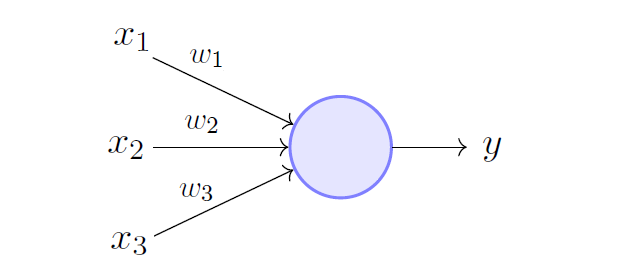
\includegraphics[width=120mm]{figures/perceptron1.png}
  \caption{Perceptron Neuron \cite{El-Amir_Hamdy_2019}}
  \label{perceptron1}
\end{figure}

A perceptron takes a number of inputs that are binary in nature and produce a single binary output \cite{Freund_Schapire_1998} ie.is this a dog? The figure \ref{perceptron1} has 3 inputs ($x_1$, $x_2$ and $x_3$) although, more or fewer inputs may be used.
Each input then is given a weight -- $w_1$, $w_2$ and $w_3$ in this case -- and the output calculated thus.

\begin{align}
  y = \begin{cases}
    0 \textrm{ if } \sum_i w_i x_i \leq \textrm{threshhold},\\
    1 \textrm{ if } \sum_i w_i x_i > \textrm{threshhold},\\
  \end{cases}
\end{align}

Used in this fashion, a perceptron can only make simple choices.
Raising the threshold makes the classification tighter while lowering it loosens the classification.
Because the output of a perceptron is binary, for more subtle distinctions, we can use the output of a perceptron to feed into the input of the next one thus creating a network that is more able to measure subtlety.

\begin{figure}[H]
  \centering
  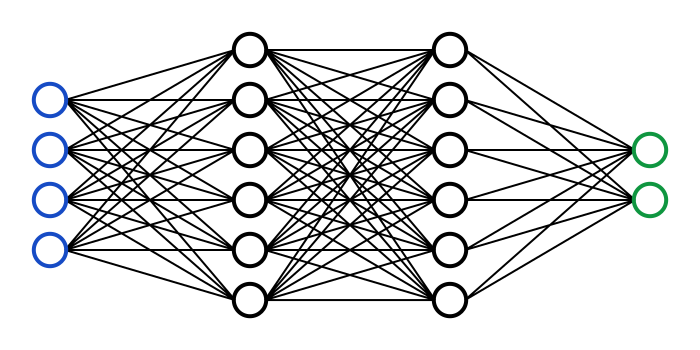
\includegraphics[width=120mm]{figures/network.png}
  \caption{Perceptron network \cite{Zhou_2020}}
  \label{network}
\end{figure}

Varying the weights of the inputs in combination with the threshold for the output allows us to get different models of classification.
The neurons in the first layer are only able to make simple decisions based on the raw input but because we use their output as the input to the second layer, the second layer can make more abstract decisions with a degree of subtlety impossible not only with one perceptron but also with even a single layer of perceptrons.
The complexity of the discrimination by the classifier increases with both the number and layers of perceptrons in the network.

With the correct weights and threshold values, we can get any binary classifier we want using a set of perceptrons.
That, however, puts us back at our original problem of classifying whether something is a dog; namely, if we knew what features to look for (i.e.\ what weights and threshold to use) it wouldn't be hard explaining to a computer what a dog was.
The true innovation comes with using learning algorithms that don't require input from the programmer to set these weights and thresholds.

  If we want to use algorithms that can adjust weights and thresholds (otherwise called biases) automatically, we need some method where a small change in the weight only causes a small change in the output.
Because perceptrons are binary, this is impossible to do with only perceptrons.

  A small change in the weight to an input to the perceptron can flip the output entirely.
While this small change in weight can make one of the outputs of the network better, it may also affect the rest of the network behave in unpredictable ways.
Going back to the dog and cat example, while changing the weight slightly may make it better at recognizing dogs, it may wreak havoc on how cats are identified.

  This is where sigmoid neurons come in.